\chapter{Pricing: Context Generation}\label{ch:pricing:-context-generation}

In this chapter we want to further expand what we have seen in the previous one.
In the general case, since we have access to many information about our clients, we can not only identify different classes of users, with different buying powers, but also understand to which class a new user belongs, based on the information we have about him (given, for example, by cookies).
The idea is to exploit this knowledge in order to charge different prices to each class and so maximize our revenue.
To do so, we will use the idea of the \textbf{context}, which will be explained in the next section.
We will then explain the differences in the environment used in this chapter, tackle the approaches we followed to create the algorithm and analyze the final results.

\section{What is a Context?}\label{sec:what-is-a-context?}
As said before, in this scenarios we have a lot of information about the users that visit our website, so we can group them together in classes.
Usually a class is identified by a single value (or subsets of values) for each feature.
The problem is that the number of classes grows exponentially with the number of features, making unfeasible the problem of defining and optimizing a single price for each class when we have many features for each user (which is the most common scenario in real cases).
A context is a partition of the feature space according to some values of the features (for example a male with age between 18 and 24 is a context), grouping together various classes.
By using contexts instead of classes, we are able to drastically reduce the number prices we have to decide, so the problem can be tackled and solved in a reasonable time.

\section{Environment, Learner and Demand Curves}\label{sec:environment,-learner-and-demand-curves}
The environment is fairly similar to the one used in Chapter 4, the only difference is that it keeps track of how many days have passed since the collected data has been analyzed, so that we know when we have enough to consider generating the new contexts.
This is possible because we know how many users will visit our website every day, so we know exactly how much data we have after each day.
We used the same demand curves as in Chapter 4, on the other hand, since we want to learn different prices now, we don't use a single learner anymore, but we create one with each new context.

\section{Campaign Scheduler}\label{sec:campaign-scheduler}
The class Campaign Scheduler acts as the main interface for our algorithm.
It stores the contexts we are currently using for the week and the information collected by our website so far in a structure indexed using the classes we have chosen.
These information are updated after each user visits the website and will then be used in the Context Generator class to decide whether to create new contexts or not.
\begin{itemize}
	\item \textit{Total Reward}: The sum of all the rewards we have obtained so far;
	\item \textit{Number of purchases}: The number of products we have actually sold;
	\item \textit{Number of users}: The number of users who have visited our website;
    \item \textit{Rewards}: An array that contains all the rewards collected so far.
\end{itemize}

\section{Our Approach to Context generation}\label{sec:our-approach-to-context-generation}
When we first approached the problem, we used a algorithm similar to that presented in class, with a greedy approach.
We start with the aggregate model, so we have only one price for all the classes, and we use it to collect data for the first week.
At the end of the week, we use this data to evaluate the features and decide if we want to split and generate new contexts.
For each feature we have yet to use to split, we compute the lower bound of the probability of the context to occur and of the expected reward.
This is because when we create a new context, we have to learn a different model, which will surely have more uncertainty with respect to the one used so far.
The lower bound is a measure of how much we are guaranteed to gain, the reward we collect in the end might be higher.

	For the lower bound of the probability we used the Hoeffding bound since the probability has limited values.

\begin{equation}
	x - \sqrt{-\frac{\log_n{d}} {2 n}}
\end{equation}
where:
\begin{itemize}
	\item $n$ : is the number of samples.
	\item $x$ : is the mean of the rewards.
	\item $d$ : is a value that defines how much confidence we want.
\end{itemize}

	For the reward, we had to use a different formula, since its values are unlimited.

\begin{equation}
	x - t \sqrt{\frac{sq} {n}}
\end{equation}
where:
\begin{itemize}
	\item $n$ : is the number of samples.
	\item $x$ and $sq$ : are the mean and variance of the real rewards.
	\item $t$ : is a value that defines how much confidence we want.
\end{itemize}

After evaluating the expected reward relative to each feature, we select the one with the highest value and compare it with the expected reward of the current model.
If it is larger or equal we create the new contexts, if not we keep the previous model and start a new week.
This process is iterated week after week, without a termination condition, because we are continuously collecting information which might change how our contexts are organized.
In the general case this algorithm does not guarantee optimality and is used to solve scenarios in which we have many features with possibly many values thanks to its performances.
On the other hand it gives us some insight on which features might be the most important in the scenario.

However our problem was quite different from the general one, so we chose a different approach: evaluating every week the entire set of possible partitions.
Since we have only two features with binary values, this process is not computationally heavy and we can use this solution with reasonable time performances.
We always start with the aggregate model to collect data, but when the time to split arrives, we evaluate all possible partitions of our feature space, using the above formulas.
This way we can either obtain the aggregate model, two or three contexts, by not splitting, splitting according to only one or both features (we would obtain four contexts, but we only have three classes).

\section{Results}\label{sec:our-result}

As in Chapter 4, we configured the experiment to both keep the same price for the day and not to and this is the reason of the two graphs.
Moreover we used the same two optimal models, the Aggregate Model, which does not know the classes of the users, and the True Evaluation, which does and chooses a single price for each of them.
This was done to compare the results of the algorithms we have built.

As we can see in figure \ref{regret5Fig}, the algorithm largely outperforms the Aggregate Model, because it knows the classes of the users and can choose a price for each of them.
In the first weeks we observe a small growth before the decrease, this is because the algorithm starts from the aggregate model and is still learning the correct prices.
We can also see that the initial growth lasts longer when we keep a daily price, because by fixing the price it takes longer to learn the curve.
On the other hand, the True Evaluation model performs better than the algorithm in the first weeks, but as time goes on the difference becomes smaller and smaller, as the algorithm learns the best prices.

\begin{figure}[!htb]
	\centering

	\begin{subfigure}[!H]{0.8\textwidth}
		\centering
		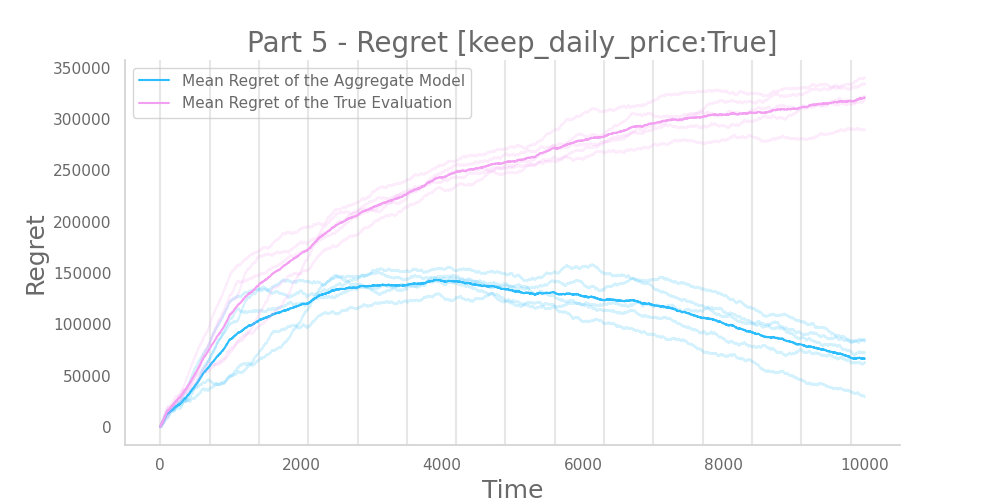
\includegraphics[width=\textwidth]{images/part5_keep-daily-priceTrue.png}
		\caption{Regret obtained proposing to the customers the same price for the entire day.}
	\end{subfigure}

	\begin{subfigure}[!H]{0.8\textwidth}
		\centering
		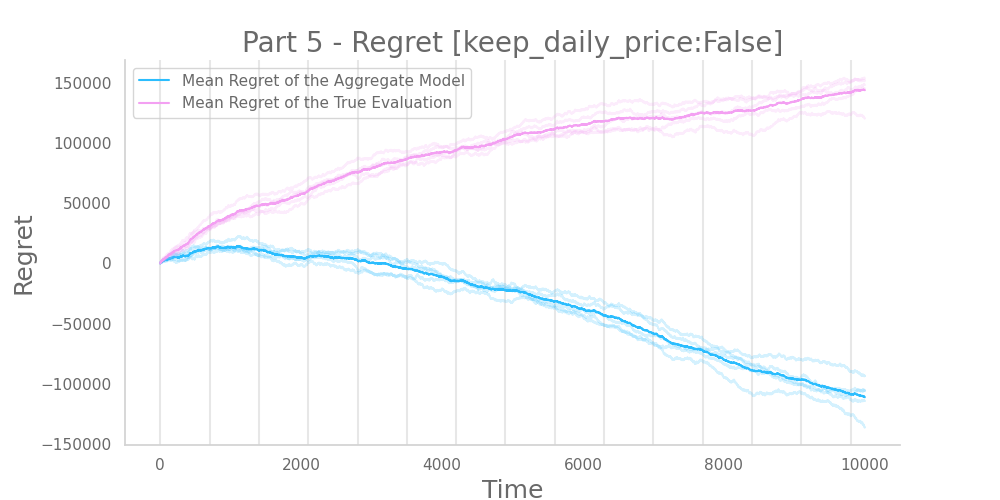
\includegraphics[width=\textwidth]{images/part5_keep-daily-priceFalse.png}
		\caption{Regret obtained proposing to the customers different prices for each visit.}
	\end{subfigure}

	\caption{Comparison between the regrets obtained during the campaign.\\
			The \textbf{Mean Regret of the Aggregate Model} (colored in \textit{blue}) is the regret computed keeping, as optimal, the area under the optimal point of the aggregate curve~\ref{demandCurvesFig}.\\
			The \textbf{Mean Regret of the True Evaluation} (colored in \textit{pink}) is the regret obtained computing the optimal value exploiting the original class of the customers.}
	\label{regret5Fig}
\end{figure}
